\documentclass[11pt, a4paper]{paper}
\usepackage{a4wide,color}

\usepackage[utf8]{inputenc}
\usepackage[T1]{fontenc}
\usepackage[frenchb]{babel}

\usepackage{graphicx}
\usepackage{amssymb}
\usepackage{hyperref}

\usepackage{amstext}
\usepackage{amsmath}

\usepackage{listings}
\usepackage{color}
\lstset{ %
  backgroundcolor=\color{white},   % choose the background color; you must add \usepackage{color} or \usepackage{xcolor}; should come as last argument
  basicstyle=\footnotesize,        % the size of the fonts that are used for the code
  breakatwhitespace=false,         % sets if automatic breaks should only happen at whitespace
  breaklines=true,                 % sets automatic line breaking
  captionpos=b,                    % sets the caption-position to bottom
  commentstyle=\color{cyan},    % comment style
  deletekeywords={...},            % if you want to delete keywords from the given language
  escapeinside={\%*}{*)},          % if you want to add LaTeX within your code
  extendedchars=true,              % lets you use non-ASCII characters; for 8-bits encodings only, does not work with UTF-8
  frame=single,	                   % adds a frame around the code
  keepspaces=true,                 % keeps spaces in text, useful for keeping indentation of code (possibly needs columns=flexible)
  keywordstyle=\color{blue},       % keyword style
  language=Octave,                 % the language of the code
  morekeywords={*,...},           % if you want to add more keywords to the set
  numbers=left,                    % where to put the line-numbers; possible values are (none, left, right)
  numbersep=5pt,                   % how far the line-numbers are from the code
  numberstyle=\tiny\color{magenta}, % the style that is used for the line-numbers
  rulecolor=\color{black},         % if not set, the frame-color may be changed on line-breaks within not-black text (e.g. comments (green here))
  showspaces=false,                % show spaces everywhere adding particular underscores; it overrides 'showstringspaces'
  showstringspaces=false,          % underline spaces within strings only
  showtabs=false,                  % show tabs within strings adding particular underscores
  stepnumber=2,                    % the step between two line-numbers. If it's 1, each line will be numbered
  stringstyle=\color{red},     % string literal style
  tabsize=2,	                   % sets default tabsize to 2 spaces
  title=\lstname                   % show the filename of files included with \lstinputlisting; also try caption instead of title
}
\usepackage{placeins}


\usepackage{framed}


\title{{\Huge Rapport de projet De Stijl}\\
{\large version \today}\\
---\\
}
\author{\color{black}
{ABDELMOUMEN Oussama (Conception, code)} \\ {GRASA Guillaume (Conception, code)}\\ {HELLO Anouk (Conception, rédaction du compte-rendu, un peu de code)} \\ {PROUVOST Chloé (Conception, rédaction du compte-rendu, un peu de code)}
}

\begin{document}

%%%%%%%%%%%%%%
% PAGE DE GARDE
\maketitle


{\color{red}
\begin{framed}
\begin{center}{\bf\Large --- Ce qu'il faut faire --- } \end{center}

{\bf Remplacez tous les textes en bleu et supprimer les textes en rouge}\\


{\bf Le rapport est à rendre en pdf et à envoyer par mail à votre encadrant de TP au plus tard le 20 janvier 2017.}\\

{\bf Vous devez aussi rendre votre code (uniquement les fichiers que vous avez écrits ou modifiés) sous la forme d'une archive (zip ou tar).}\\

Vous pouvez utiliser word ou un autre logiciel d'édition pour rédiger ce rapport, par contre vous devez  {\bf obligatoirement} respecter la structure décrite ici.\\


Critères d'évaluation :
\begin{itemize}
	\item Qualité rédactionnelle,
	\item Exhaustivité et justesse des règles de codage,
	\item Qualité de la conception (clarté, respect de la syntaxe, exhaustivité, justesse),
	\item Qualité des explications,
	\item Respect des règles dans la production du code\\
\end{itemize}

Compétences évaluées :
\begin{itemize}
	\item rédaction et communication sur un dossier de conception
	\item concevoir une application concurrente temps réel
	\item analyser une conception
	\item passer d'un modèle de conception à une implémentation
	\item écriture de code C et utilisation de primitives au niveau système
\end{itemize}
\end{framed}
}

%%%%%%%%%%%%%%
% DEBUT DU RAPPORT
\newpage


%%%%%%%%%%%%%%
% CONCEPTION
\section{Conception}

{\color{red} Mettez dans cette partie tous les éléments de votre conception en particulier vos diagrammes AADL (vue globale du système et détails des threads). Cette partie doit être auto-suffisante pour comprendre votre application.

Pour faciliter la lecture des schémas, vous allez présenter votre conception en trois parties, l'une focalisée sur la communication entre le moniteur et le superviseur, la seconde consacrée au contrôle du robot et la troisième au traitement vidéo.

{\bf La partie de gestion automatique d'une mission du robot sera à part pour ceux l'ayant traitée.}

Si vous le souhaitez, au lieu de dessiner vos diagrammes sous un éditeur, vous pouvez joindre un scan de vos schémas — ils doivent être lisibles et propres.}

% VUE GENERAL DU SYSTEME
\subsection{Diagramme fonctionnel général}

{\color{red} Mettez ici un diagramme fonctionnel qui présente les principaux blocs de votre conception. Pour cela, inspirez vous du diagramme ci-dessous (fig.~\ref{fig:diag_fonc_gen}) en indiquant pour chaque groupe de threads les données et ports partagés. La figure~\ref{fig:diag_fonc_gen} a été réalisée à partir du document de conception. {\bf Vous devez absolument conserver le découpage en trois groupes de threads ({\tt th\_group\_gestion\_moniteur}, {\tt th\_group\_gestion\_robot}, {\tt th\_group\_vision}).}}

\begin{figure}[htbp]
\label{fig:diag_fonc_gen}
\begin{center}
{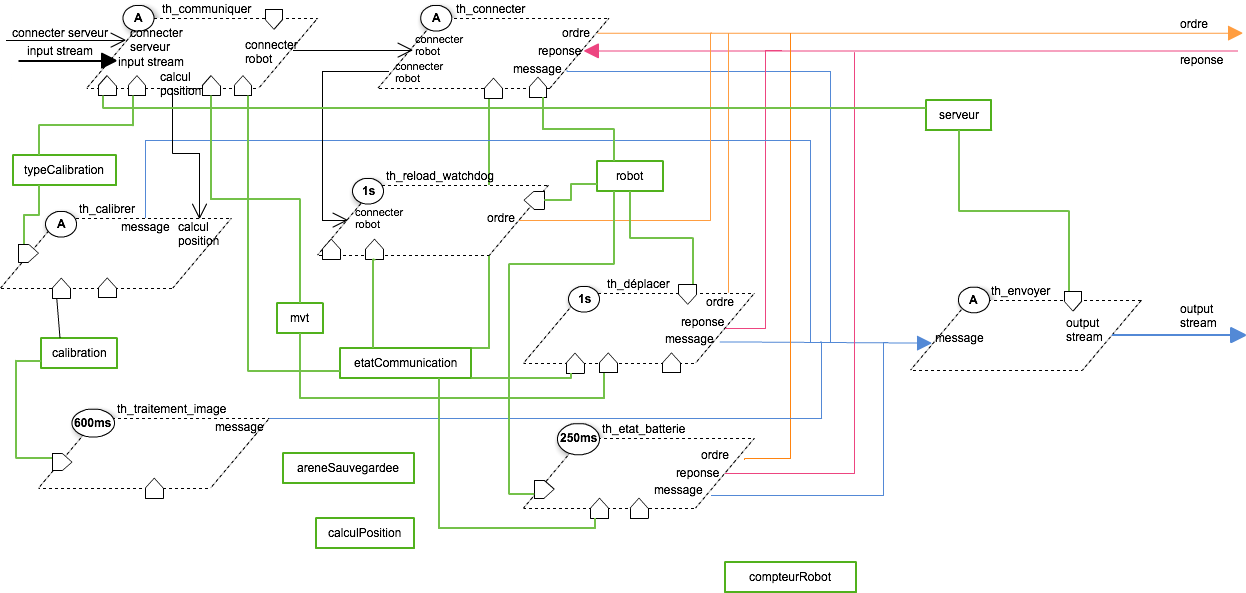
\includegraphics[scale=.4]{./figures/grosdiagramme}}
{\caption{Diagramme fonctionnel du système}}
\end{center}
\end{figure}
\FloatBarrier

% DIAGRAMME FONCTIONNEL GT MONITEUR
\subsection{Groupe de threads gestion du moniteur}

{\color{red}Placez ici :
\begin{itemize}
\item le diagramme fonctionnel en AADL décrivant le groupe de threads de gestion du moniteur (voir exemple de la figure~\ref{fig:diag_fonc_moniteur} réalisée à partir du dossier de conception),
\item remplir le tableau~\ref{tab:gt_moniteur} pour expliquer le rôle de chacun des threads,
\item les diagrammes d'activité de chaque thread de ce groupe.
\end{itemize}

Décrivez tous les éléments (paramètres, variables, etc.) qui vous semblent pertinents pour comprendre les diagrammes.}

% DIAGRAMME FONCTIONNEL GT MONITEUR
\subsubsection{Diagramme fonctionnel du groupe gestion du moniteur}

{\color{red} Exemple de diagramme fonctionnel pour le groupe de thread de gestion du moniteur. Mettez à jour ce diagramme avec votre conception.}

\begin{figure}[htbp]
\label{fig:diag_fonc_moniteur}
\begin{center}
{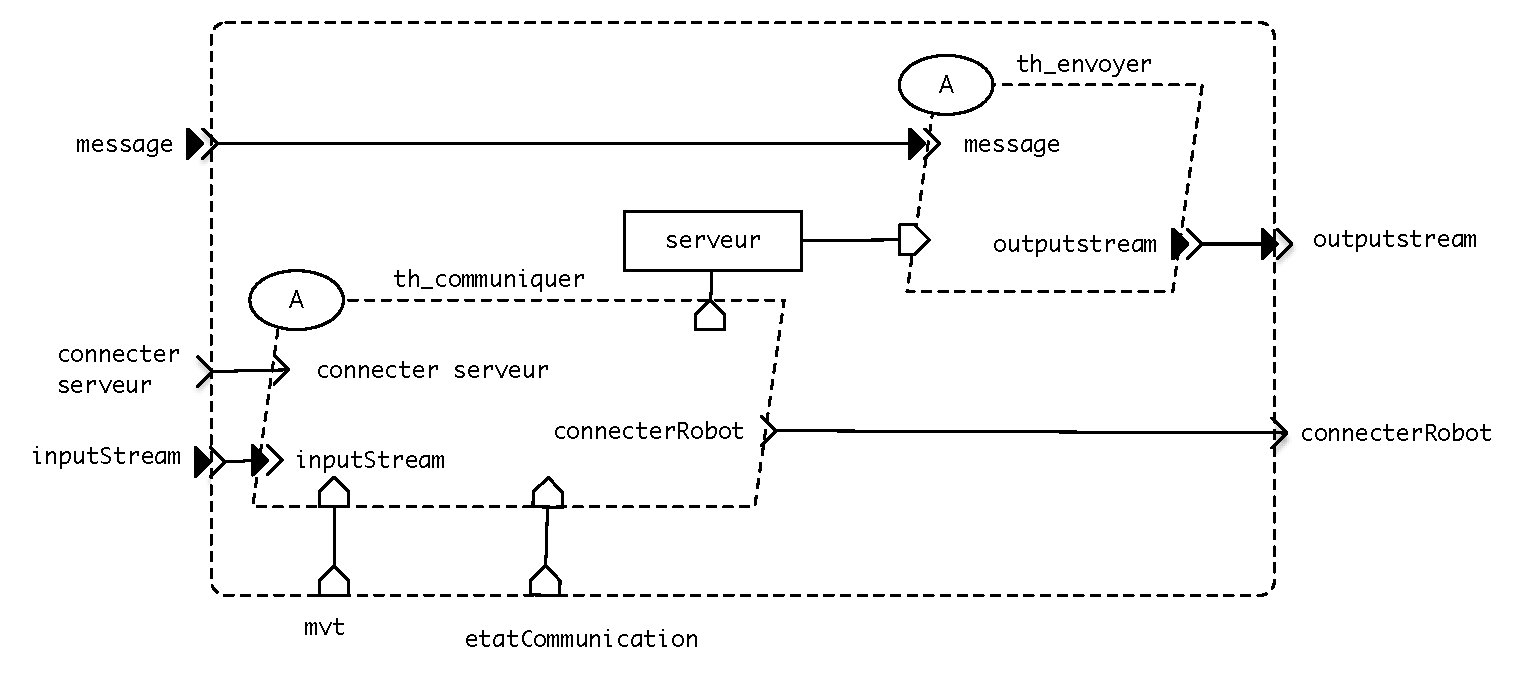
\includegraphics[scale=.5]{./figures-pdf/diag_fonc_moniteur}}
{\caption{Diagramme fonctionnel du groupe de threads gestion du moniteur}}
\end{center}
\end{figure}
\FloatBarrier

% DESCRIPTION THREADS GT MONITEUR
\subsubsection{Description des threads  du groupe gestion du moniteur}
{\color{red} Remplissez le tableau ci-dessous pour expliquer le rôle de chaque thread et donner son niveau de priorité.}


\begin{table}[htp]
\caption{Description des threads du groupe {\tt th\_group\_gestion\_moniteur}}
\begin{center}
\begin{tabular}{|p{3cm}|p{8.5cm}|p{2cm}|}
\hline
\bf Nom du thread &	\bf Rôle &	\bf Priorité \\
\hline
\hline
\color{black}thCommuniquer	& \color{black}Prend en charge les messages entrants depuis le moniteur & \color{black}50\\
\hline
\color{black}thEnvoyer	& \color{black}Envoi l'ensemble des messages du superviseur au moniteur & \color{black}55\\
\hline
\color{black}... &	\color{black}... &	\color{black}...\\
\hline
\end{tabular}
\end{center}
\label{tab:gt_moniteur}
\end{table}%

% DIAGRAMMES D'ACTIVITE GT MONITEUR
\subsubsection{Diagrammes d'activité  du groupe gestion du moniteur}
{\color{red}Décrivez le comportement de chacun de vos threads avec des diagrammes d'activité. Apportez les explications qui vous semblent nécessaires pour comprendre votre conception. A titre d'exemple les diagrammes fonctionnels tirés du document de conception sont remis.}

\begin{figure}[htbp]
\label{fig:act_communiquer}
\begin{center}
{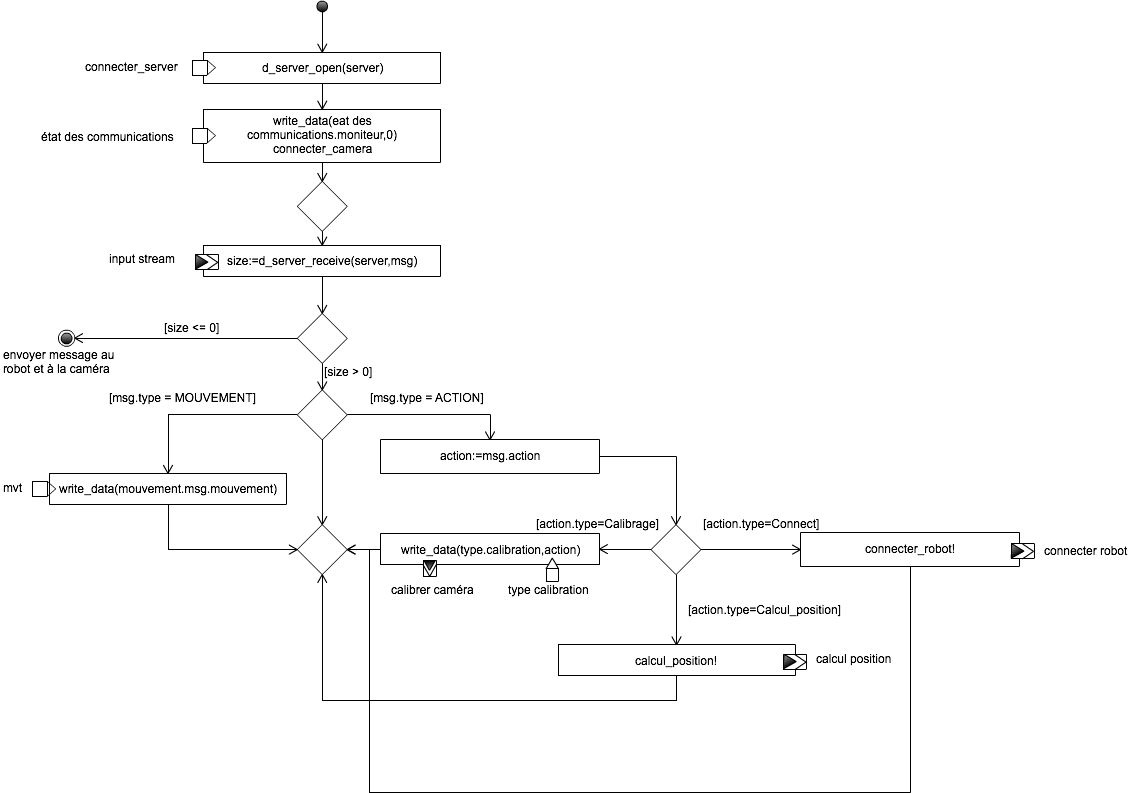
\includegraphics[scale=.4]{./figures/communiquer}}
{\caption{Diagramme d'activité du thread {\tt th\_communiquer}}}
\end{center}
\end{figure}
\FloatBarrier

\begin{figure}[htbp]
\label{fig:act_envoyer}
\begin{center}
{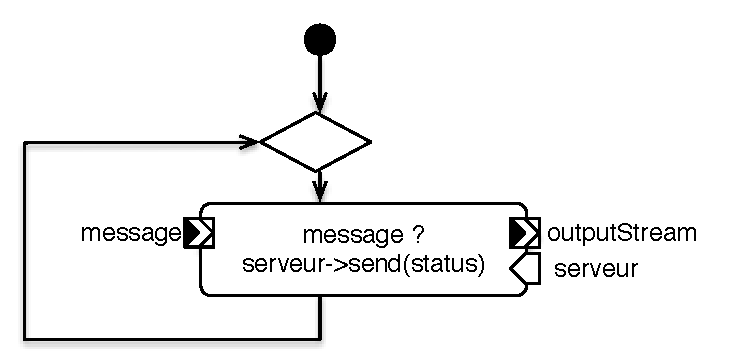
\includegraphics[scale=.5]{./figures-pdf/act_envoyer}}
{\caption{Diagramme d'activité du thread {\tt th\_envoyer}}}
\end{center}
\end{figure}
\FloatBarrier

% DIAGRAMME FONCTIONNEL GT ROBOT
\subsection{Groupe de threads gestion du robot}

% DIAGRAMME FONCTIONNEL GT ROBOT
\subsubsection{Diagramme fonctionnel du groupe gestion robot}
{\color{blue} Ajoutez le diagramme fonctionnel du groupe de threads de gestion du robot.}

% DESCRIPTION THREADS GT ROBOT
\subsubsection{Description des threads du groupe gestion robot}



\begin{table}[htp]
\caption{Description des threads du groupe {\tt th\_group\_gestion\_robot}}
\begin{center}
\begin{tabular}{|p{3cm}|p{8.5cm}|p{2cm}|}
\hline
\bf Nom du thread &	\bf Rôle &	\bf Priorité \\
\hline
\hline
\color{black}thConnecter &	\color{black}Ouvre la communication avec le robot &	\color{black}50\\
\hline
\color{black}thReloadWatchdog &	\color{black}Surveille la perte de communication entre le robot et le superviseur &	\color{black}45\\
\hline
\color{black}thDeplacer &	\color{black}Envoi des ordres de déplacement au robot &	\color{black}40\\
\hline
\color{black}thEtatBatterie &	\color{black}Surveille l'état de la batterie du robot et l'envoi au moniteur via le thread thEnvoyer &	\color{black}10\\
\hline
\end{tabular}
\end{center}
\label{tab:gt_moniteur}
\end{table}%
\FloatBarrier

% DIAGRAMMES D'ACTIVITE GT ROBOT
\subsubsection{Diagrammes d'activité du groupe robot}

\begin{figure}[htbp]
\label{fig:act_communiquer}
\begin{center}
{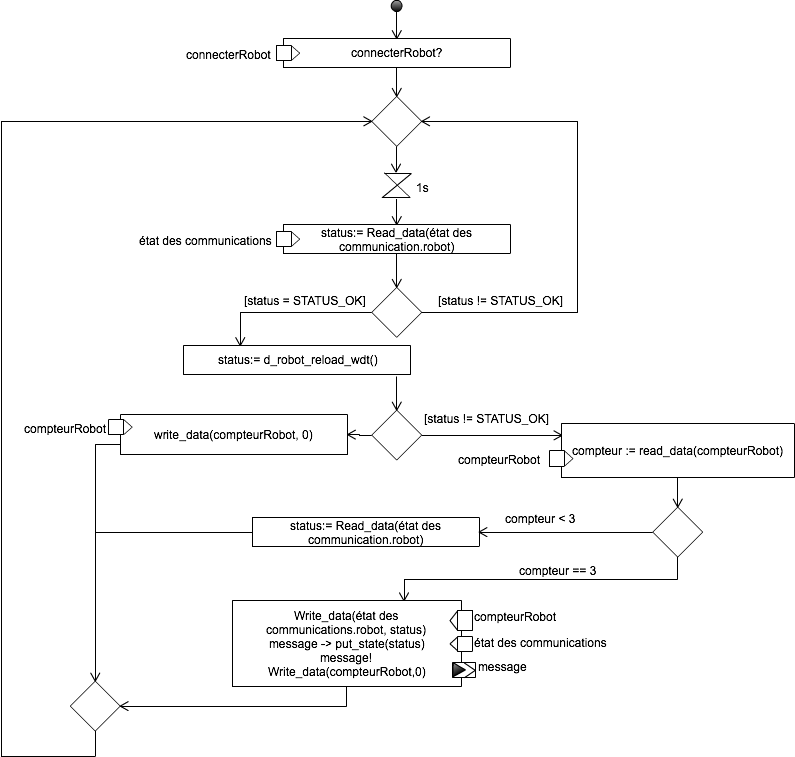
\includegraphics[scale=.4]{./figures/watchdog}}
{\caption{Diagramme d'activité du thread thReloadWatchdog}}
\end{center}
\end{figure}
{\color{black}On attend que le robot soit connecté pour lui envoyer l'ordre de rechargement du watchdog.}

\begin{figure}[htbp]
\label{fig:act_communiquer}
\begin{center}
{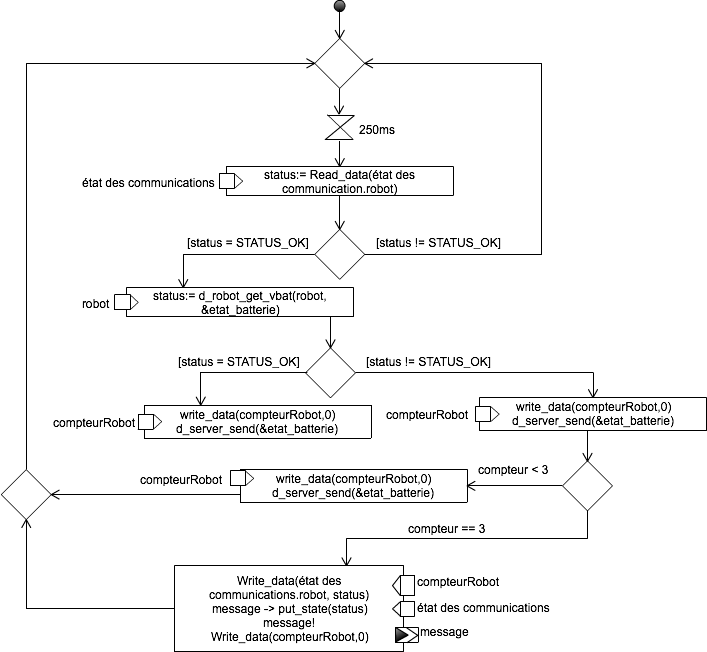
\includegraphics[scale=.4]{./figures/etat_batterie}}
{\caption{Diagramme d'activité du thread thEtatBatterie}}
\end{center}
\end{figure}
\FloatBarrier

\begin{figure}[htbp]
\label{fig:act_communiquer}
\begin{center}
{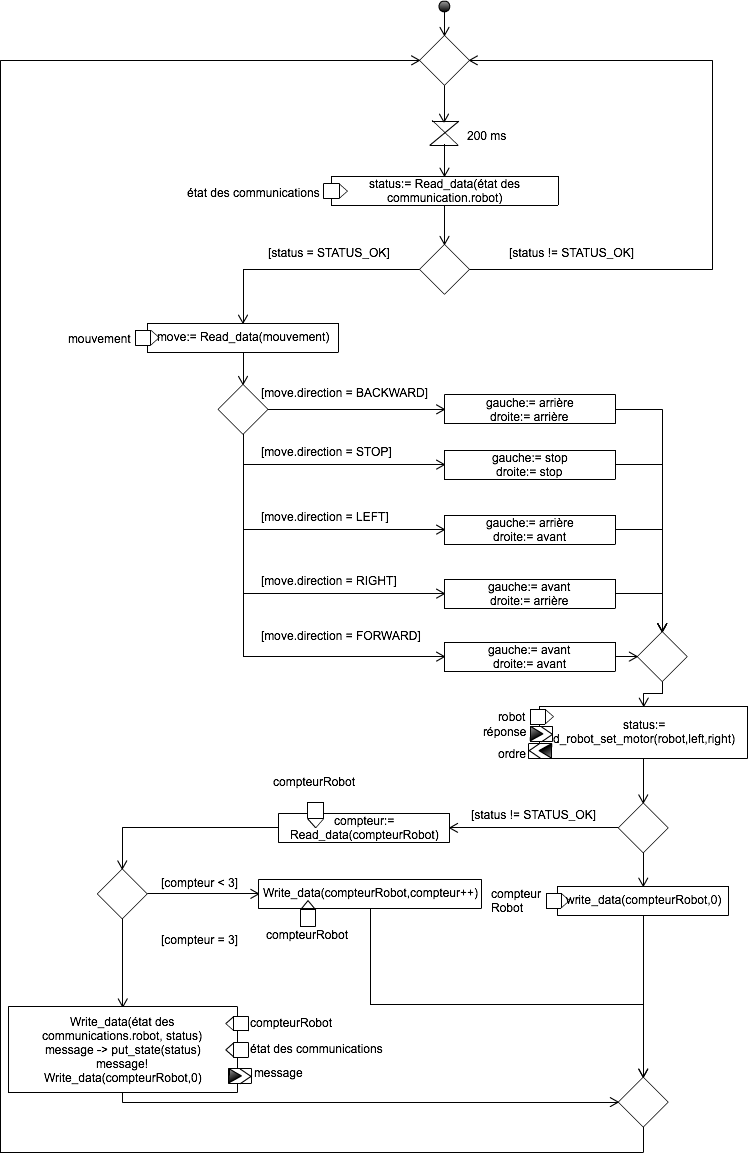
\includegraphics[scale=.4]{./figures/deplacer}}
{\caption{Diagramme d'activité du thread thDeplacer}}
\end{center}
\end{figure}
\FloatBarrier


% DIAGRAMME FONCTIONNEL GT VISION
\subsection{Groupe de threads vision}

% DIAGRAMME FONCTIONNEL GT VISION
\subsubsection{Diagramme fonctionnel du groupe vision}

{\color{blue} Ajoutez le diagramme fonctionnel du groupe de threads de vision.}

% DESCRIPTION THREADS GT VISION
\subsubsection{Description des threads du groupe vision}
{\color{red} Remplissez le tableau ci-dessous pour expliquer le rôle de chaque thread et donner son niveau de priorité.}


\begin{table}[htp]
\caption{Description des threads du groupe {\tt th\_group\_vision}}
\begin{center}
\begin{tabular}{|p{3cm}|p{8.5cm}|p{2cm}|}
\hline
\bf Nom du thread &	\bf Rôle &	\bf Priorité \\
\hline
\hline
\color{black}thTraitementImage &	\color{black}Capture une image, si l'utilisateur souhaite la position du robot, il la dessine sur cette image, compresse l'image et l'envoi en message. Si il ne veux pas la position il compresse l'image puis l'envoi en message. Il ne peut pas s'exécuter si il y a une calibration. &	\color{blue}30\\
\hline
\color{black}thCalibration &	\color{black}Détection de l'arène, l'utilisateur doit valider la calibration ou redemander une détection &	\color{blue}35\\
\hline
\end{tabular}
\end{center}
\label{tab:gt_moniteur}
\end{table}%
\FloatBarrier

% DIAGRAMMES D'ACTIVITE GT VISION
\subsubsection{Diagrammes d'activité du groupe vision}
{\color{blue}Décrivez le comportement de chacun de vos threads avec des diagrammes d'activité. Apportez les explications qui vous semblent nécessaires pour comprendre votre conception.}

\begin{figure}[htbp]
\label{fig:act_calibration}
\begin{center}
{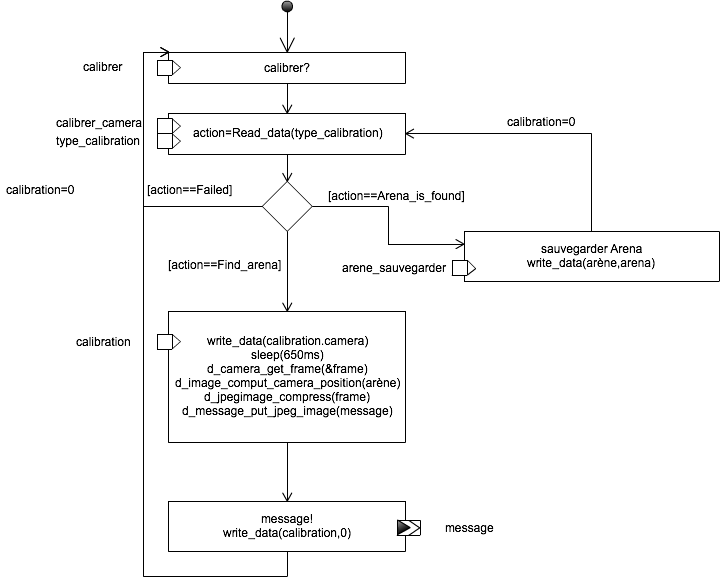
\includegraphics[scale=.4]{./figures/calibration}}
{\caption{Diagramme d'activité du thread {\tt thCalibration}}}
\end{center}
\end{figure}
\FloatBarrier

\begin{figure}[htbp]
\label{fig:act_calibration}
\begin{center}
{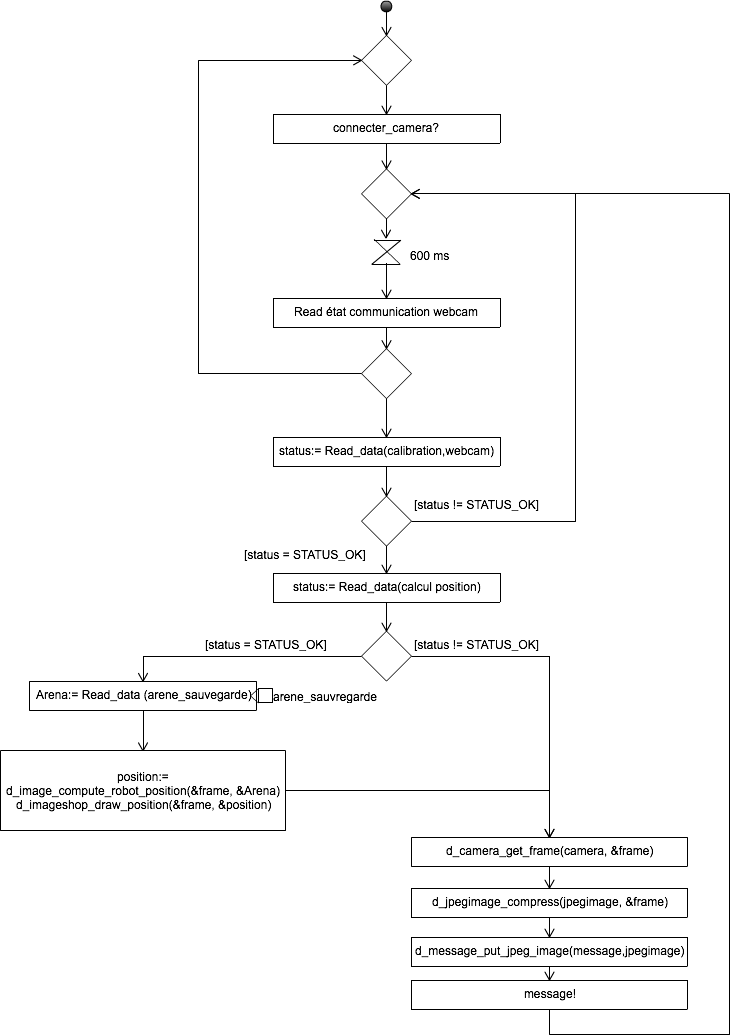
\includegraphics[scale=.4]{./figures/traitement_image}}
{\caption{Diagramme d'activité du thread {\tt thTraitementImage}}}
\end{center}
\end{figure}
\FloatBarrier

\newpage

%%%%%%%%%%%%%%%
% ANALYSE ET VALIDATION
\section{Analyse et validation de la conception}

{\color{red}
Pour les trois exigences suivantes montrer en quoi votre conception permet d’y répondre. }

% EXIGENCE EXEMPLE
{\color{red} \subsection*{Exemple de ce qui est attendu}

Voici un exemple avec pour exigence : \og une fois la communication établie avec le robot, les ordre de mouvement sélectionnés par l'utilisateur sur le moniteur sont transmis au robot.\fg\ 

Il faut justifier à travers la conception que cette exigence est bien prise en considération et estimer le temps maximum que peut prendre la transmission d'un ordre.

Pour illustrer cela, je m'appuie sur la première conception du système qui est faite  dans le document \og Dossier de conception \fg.

{\bf Justification} : une fois la communication établie, les ordres de l'utilisateur sont reçus par le superviseur via le port {\tt connecter\_serveur} du thread {\tt th\_communiquer} (attente de la fonction {\tt d\_server\_receive} sur la figure 4).

Le diagramme d'activité du thread (fig. 4) montre qu'à la réception d'un message de type MOUVEMENT la valeur qu'il porte est écrite dans la donnée partagée {\tt mouvement}. 

Cette donnée est lue périodiquement par le thread {\tt th\_deplacer}. Son diagramme d'activité (fig. 7) montre qu'en fonction de la valeur de la donnée {\tt mouvement} les variables  internes à {\tt th\_deplacer} nommées {\tt gauche} et {\tt droite} sont mises à jour pour ensuite être transmises au robot via l'appel à la fonction {\tt d\_robot\_set\_motor}.

{\bf Estimation du temps de traitement} : la figure~\ref{fig:seq} montre la séquence d'exécution la plus désavantageuse pour la prise en compte d'un ordre de mouvement. L'utilisateur commence par sélectionner son ordre sur l'interface graphique qui ajoute un délai de 200~ms avant de le transmettre au superviseur (on ignore ici les délais réseaux). Le thread {\tt th\_communiquer} étant le plus prioritaire, il traite immédiatement le message (on remarque par exemple sur la figure la préemption du thread {\tt th\_deplacer}). Le temps de traitement de {\tt th\_communiquer} est estimer à 1~ms d'après le document \og Dossier de conception \fg.

La pire des situations est une exécution du thread {\tt th\_deplacer} juste avant la réception du message de mouvement qui devra attendre 1 seconde avant de lire la nouvelle valeur de {\tt mouvement}. Le temps de transmission de l'ordre au robot a été estimé à 41~ms (voir p.~12 du document \og Dossier de conception \fg).

Nous avons donc un délai possible de l'ordre de 0.2+0.001+1+0.041 = 1.242~s entre la sélection d'un mouvement par l'utilisateur et sa réception par le robot.

\begin{figure}[htbp]
\begin{center}
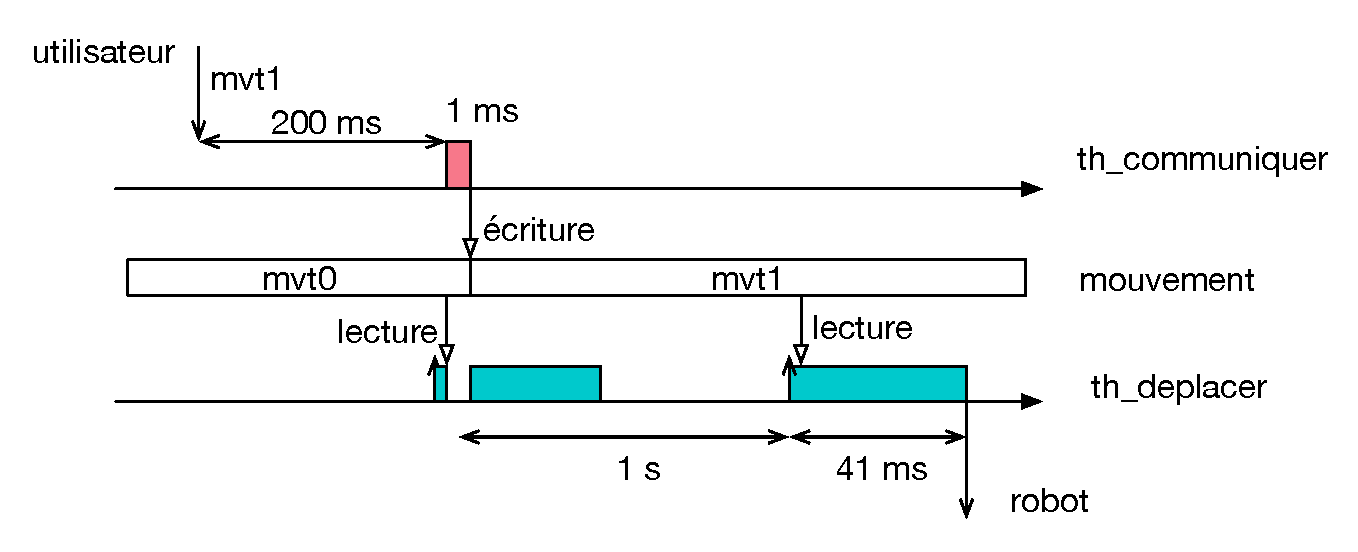
\includegraphics[scale=0.6]{./figures-pdf/sequence}
\caption{\color{red}Exemple de pire séquence d'exécution pour la transmission d'un ordre de mouvement au robot.}
\label{fig:seq}
\end{center}
\end{figure}
}

% EXIGENCE 1
\subsection{Exigence 1 : En cas de perte de communication entre le robot et le superviseur, le robot est stoppé et le nouvel état est signalé à l'utilisateur via le moniteur.}

{\color{black} Toutes les secondes, le superviseur envoie un ordre de rechargement du watchdog au robot pour éviter qu'il expire. Car si il expire, un compteur local au robot s'incrémente et lorsqu'il atteint 7, le robot s'arrête et doit être redémarré manuellement. 

{\color{blue} Fournissez un chronogramme (ou un diagramme de séquence si vous préférez) avec l’ordonnancement de votre système et estimer la plus grande durée entre l'instant où la communication est perdue et l'instant où l'utilisateur en est informé.}

% EXIGENCE 2
\subsection{Exigence 2 : La communication entre le robot et le superviseur est déclarée perdue si et seulement si trois échecs successifs de communication entre le robot et le superviseur surviennent.}

{\color{black} Quand le superviseur donne un ordre au robot, il répond en envoyant son status. Si le superviseur ne reçoit aucune réponse, un compteur global s'incrémente. S'il atteint 3, on déclare que la connexion est perdue et on en informe le moniteur via la file de messages. De même, si le robot ne répond pas à l'ordre de rechargement du watchdog ou à l'ordre de réception du nouveau niveau de la batterie, le compteur global, qui est partagé entre tous les threads qui communiquent avec le robot, s'incrémente. Si le robot répond, le compteur se remet à 0. }

% EXIGENCE 3
\subsection{Exigence 3 : 
L'image qui est  affichée sur le moniteur ne doit pas être plus vieille que 600~ms (différence de temps entre la capture de l'image et son affichage sur le moniteur).}

{\color{blue} Expliquez en vous appuyant sur votre conception comment vous garantissez que cette exigence est toujours respectée. \\}
{\color{black} thread traitement image, periode 600ms. Il a une petite priorité. 4*40ms + 250ms < 600 ms \\}
{\color{blue} Fournissez un chronogramme (ou un diagramme de séquence si vous préférez) avec l’ordonnancement de votre système qui montre en quoi cela répond bien à cette exigence. Expliquez.}


%%%%%%%%%%%%%%%%%%%
% TRANSFORMATION AADL2XENO
\section{Transformation AADL2XENO}
 
 {\color{red} Cette section est consacrée aux moyens pour passer d'un modèle AADL au code. Pour chacun des éléments AADL, vous allez expliquer {\bf comment le traduire en C} et quels {\bf services de Xenomai} vous avez utilisés {\bf en expliquant ce qu'il fait}. N'hésitez pas à illustrer avec des extraits de code.}
 
% THREAD
\subsection{Thread}
% INSTANCIATION THREAD
\subsubsection{Instanciation et démarrage}
{\color{black} Un thread AADL est instancié en C par une tâche ({\tt RT\_TASK}) Xenomai.  Pour cela, une structure {\tt RT\_TASK} est déclarée comme variable globale pour chaque tâche.

Le service {\tt rt\_task\_create} est utilisé pour créer la tâche, c'est-à-dire réserver son space mémoire et la déclarer au noyau, et {\tt rt\_task\_start} pour lancer l'exécution de la tâche.}

% CODE THREAD
\subsubsection{Code à exécuter}
 {\color{black} Sous Xenomai, le lien entre le thread et le traitement à exécuter se fait grâce à l'appel de la fonction {\tt rt\_task\_start} qui prend en argument une structure {\tt RT\_TASK} et le thread à exécuter. Par exemple pour lancer le thread connecter, on appelle la fonction de la manière suivante : {\tt rt\_task\_start}(\&tconnect, \&connecter, NULL).}

% PRIORITE THREAD
\subsubsection{Niveau de priorités}
 {\color{black} Expliquer comment vous fixez sous Xenomai le niveau de priorité d'un thread AADL. On déclare d'abord en variable globale le niveau de priorité que l'on souhaite attribuer au thread, puis on donne ce niveau de priorité en argument lors de la création de ce thread avec le service {\tt rt\_task\_create}}. Exemple : {\tt rt\_task\_create}(\&tenvoyer, NULL, 0, PRIORITY\_TENVOYER, 0) où PRIORITY\_TENVOYER est un entier déclaré en variable globale. On affecte des entiers 10, 20, 30, 40, etc aux niveaux de priorité pour qu'en cas d'évolution de la spécification, l'impact soit moins lourd.}

% PERIODICITE THREAD
\subsubsection{Activation périodique}
 {\color{black} On rend périodique l'activation d'un thread AADL sous Xenomai grâce à deux fonctions : {\tt rt\_task\_set\_periodic} qui permet de fixer la période de la tâche et {\tt rt\_task\_wait\_period} qui permet de libérer le processeur quand la tâche a terminé son traitement et doit attendre la prochaine période.}

% THREAD EVENEMENTIEL
\subsubsection{Activation événementielle}
 {\color{blue} Expliquer les moyens mis en {\oe}uvre dans l'implémentation sous Xenomai pour gérer les activations événementielles d'un thread AADL.}
\\Les moyens mis en {\oe}uvre sont : les sémaphores.

% PORT D'EVENEMENT
\subsection{Port d’événement}

% INSTANCIATION PORT D'EVENEMENT
\subsubsection{Instanciation}
 {\color{blue} Comment avez-vous instancié un port d'événement ?}
\\On instancie les sémaphores à la valeur 0 dans le main.c grâce à la fonction rt\_sem\_create(\&semEvent..,0,..) et en déclarant en extern dans le global.h la sémaphore : extern RT\_SEM semEvent et dans le global.c RT\_SEM semEvent.

% ENVOI PORT D'EVENEMENT
\subsubsection{Envoi d’un événement}
 {\color{blue} Quels services ont été employés pour envoyer un événement ?}
\\Pour envoyer un événement on libère le sémaphore associé à un l'événement en incrémentant sa valeur de 1 grâce à la fonction rt\_sem\_v(\&semEvent, INFINITE). 

% RECEPTION PORT D'EVENEMENT
\subsubsection{Réception d’un événement}
 {\color{blue} Comment se fait la synchronisation sur événement ?}
\\La synchronisation sur un événement se fait avec l'acquisition de la sémaphore de l'événement qui décrémente sa valeur de 1 grâce à la fonction rt\_sem\_p(\&semEvent).

% DONNEE PARTAGEE
\subsection{Donnée partagée}

% INSTANCIATION DONNEE PARTAGEE
\subsubsection{Instanciation}
 {\color{black} Pour instancier une donnée partagée, on déclare la donnée en global puis on crée un mutex associé à cette donnée grâce à la fonction {\tt rt\_mutex\_create} qui prend en argument une structure RT\_MUTEX. Cela permettra d'éviter l'accès simultané à la donnée partagée par plusieurs processus.}

% LECTURE/ECRITURE DONNEE PARTAGEE
\subsubsection{Accès en lecture et écriture}
 {\color{black} Pour accéder en lecture ou en écriture à une donnée partagée, il faut verrouiller le mutex associé à la donnée. Pour cela on appelle la fonction {\tt rt\_mutex\_acquire}. Pour relâcher la donnée, il faut déverrouiller le mutex associé grâce à la fonction {\tt rt\_mutex\_acquire}. }

% PORT D'EVENEMENT-DONNEES
\subsection{Ports d’événement-données}

% INSTANCIATION PORT D'EVENEMENT-DONNEES
\subsubsection{Instanciation}
 {\color{blue} Donnez la solution retenue pour implémenter un port d'événement-données avec Xenomai.}
\\L'instanciation des ports d'événement-données avec Xenomai est faite grâce à l'instantciation de la structure serveur (Pas sur.. ? ) 

% ENVOI PORT D'EVENEMENT-DONNEES
\subsubsection{Envoi d’une donnée}
 {\color{blue} Quels services avez-vous employés pour envoyer des données ?}
\\Pour envoyer des données on appelle la fonction appartenant à la structure serveur qui a déjà été implémentée : {server->send(serveur,msg)}

% RECEPTION PORT D'EVENEMENT-DONNEES
\subsubsection{Réception d’une donnée}
 {\color{blue} Quels services avez-vous employé pour recevoir des données ?}
\\Pareil grâce à la fonction receive de la structure server : server->receive(server,msg)

%%%%%%%%%%%%%%%%%%%%
% EXEMPLE DE TRANSFORMATION
\section{Application de la transformation AADL2Xenomai}

{\color{blue} Vous trouverez à la fin de ce document (voir annexe~\ref{ann:conception}) une application très simple modélisée en AADL. Mettez ici le code de cette application en suivant scrupuleusement vos règles.

Ne mettez pas vos fichiers d'en-tête (sauf des extraits importants si nécessaire) et structurer le plus simplement le code. L'important est de montrer la cohérence entre les règles énoncées ci-dessus et le code que vous produisez sur l'exemple.}



%%%%%%%%%%%%%%
% EXEMPLE A TRADUIRE
\newpage
\appendix
\section{Cas d'étude à traduire}
\label{ann:conception}
\begin{itemize}
\item \large{\bf fonctions.c}

\lstset{language=C} 
\begin{lstlisting}

void th_controler (void *arg)
{

  int new_osd;
  int nouvelle_commande;

  rt_printf ("th_controler :  initialisation du systeme\n");
  initialiser_le_systeme();

  t_printf("th_controler : Demarrage des threads\n");   //On donne suffisament de ressources pour que les 2 autres threads puissent demarrer

  rt_sem_v(&semDemarrage, TM_INFINITE);
  rt_sem_v(&semDemarrage, TM_INFINITE);

  rt_printf("th_controler : Debut de l'execution de periodique a 80s\n");
  rt_task_set_periodic(NULL, TM_NOW, 80000000000);


  while (1)
    {

    rt_mutex_acquire (&mutexCommande, TM_INFINITE); //lecture de la nouvelle commande
    nouvelle_commande = commande;
    rt_mutex_release (&mutexCommande);

    new_osd = calcul_osd(nouvelle_commande); //calcul du nouvel OSD

    rt_mutex_acquire (&mutexOSDBuff, TM_INFINITE); //modification de OSD Buffer
    osdBuffer = new_osd;
    rt_mutex_release (&mutexOSDBuff);

    rt_mutex_acquire (&mutexOSD, TM_INFINITE); //modification de OSD
    osd = new_osd;
    rt_mutex_release (&mutexOSD);

    rt_task_wait_period(NULL);
    rt_printf("th_controler  : Activation periodique\n");

	 }
}


void th_capture (void *arg)
{

  DImage *image_capturee;
  DMessage *message;
  DJpegimage *jpegimage;


  rt_printf ("th_capture :  en attente de demarrage\n");
  rt_sem_p(&semDemarrage, TM_INFINITE);

  rt_printf("th_capture : Demarrage Succes\n");


  while (1)
    {
        image_capturee = d_new_image();
        image_capturee = acquisition_image(image);

        jpegimage = d_new_jpegimage();
        d_jpegimage_compress(jpegimage,frame);
        message = d_new_message();
        d_message_put_jpeg_image(message,jpegimage);

        rt_printf("th_capture  : Envoie de l'image capturee \n");
        if (write_in_queue(&queueMsgGUI, message, sizeof (DMessage)) < 0) {message->free(message);}

    }
}


void th_display (void *arg)
{

  DImage *image_capturee;
  DMessage *message;
  DJpegimage *jpegimage;


  rt_printf ("th_display :  en attente de demarrage\n");
  rt_sem_p(&semDemarrage, TM_INFINITE);

  rt_printf("th_display : Demarrage Succes\n");


  while (1)
    {
        if ((err = rt_queue_read (&queueMsgGUI, &image_capturee, sizeof (DMessage), TM_INFINITE)) >= 0) {

            rt_mutex_acquire (&mutexOSD, TM_INFINITE); //osd_var := Read_data(osd)
            osd_var = osd;
            rt_mutex_release (&mutexOSD);

            img = encode(image_capturee, osd_var);

            rt_mutex_acquire (&mutexBufferEcran, TM_INFINITE); //osd_var := Read_data(osd)
            buffer_ecran = img;
            rt_mutex_release (&mutexBufferEcran);
      }
      else  {rt_printf ("th_display : Error msg queue write: %s\n", strerror (-err));}

    }
}

\end{lstlisting}

\item \large{\bf global.h}

\lstset{language=C} 
\begin{lstlisting}
extern RT_TASK th_controler;
extern RT_TASK th_display;
extern RT_TASK th_capture;


 /* @descripteurs des mutex */
 extern RT_MUTEX mutexCommande;
 extern RT_MUTEX mutexOSDBuff;
 extern RT_MUTEX mutexOSD;
 extern RT_MUTEX mutexBufferEcran;


 /* @descripteurs des sempahore */
 extern RT_SEM semDemarrage;
 extern RT_SEM semImageCapturee;


 /* @descripteurs des files de messages */
 extern RT_QUEUE queueMsgGUI;


 /* @variables partagees */
 extern int osdbuffer;
 extern int osd;
 extern int commande;
 extern int buffer_ecran;


 /* @constantes */
 extern int MSG_QUEUE_SIZE;
 extern int PRIORITY_THCONTROLER;
 extern int PRIORITY_THCAPTURE;
 extern int PRIORITY_THDISPLAY;
\end{lstlisting}


\item \large{\bf global.c}

\lstset{language=C} 
\begin{lstlisting}
 RT_TASK th_controler;
 RT_TASK th_display;
 RT_TASK th_capture;

 RT_MUTEX mutexCommande;
 RT_MUTEX mutexOSDBuff;
 RT_MUTEX mutexOSD;
 RT_MUTEX mutexBufferEcran;

 RT_SEM semDemarrage;
 RT_SEM semImageCapturee;

 RT_QUEUE queueMsgGUI;


  int MSG_QUEUE_SIZE = 10;

  int PRIORITY_THCONTROLER = 60;
  int PRIORITY_THDISPLAY = 70;
  int PRIORITY_THCAPTURE = 80
\end{lstlisting}

\item \large{\bf main.c}

\lstset{language=C} 
\begin{lstlisting}
void initStruct(void) {
    int err;
    /* Creation des mutex */
    if (err = rt_mutex_create(&mutexOSDBuff, NULL)) {
        rt_printf("Error mutex create: %s\n", strerror(-err));
        exit(EXIT_FAILURE);
    }
    if (err = rt_mutex_create(&mutexOSD, NULL)) {
        rt_printf("Error mutex create: %s\n", strerror(-err));
        exit(EXIT_FAILURE);
    }

    if (err = rt_mutex_create(&mutexCommande, NULL)) {
        rt_printf("Error mutex create: %s\n", strerror(-err));
        exit(EXIT_FAILURE);
    }

    if (err = rt_mutex_create(&mutexCommande, NULL)) {
        rt_printf("Error mutex create: %s\n", strerror(-err));
        exit(EXIT_FAILURE);
    }


    /* Creation du semaphore */
    if (err = rt_sem_create(&semDemarrage, NULL, 0, S_FIFO)) {
        rt_printf("Error semaphore create: %s\n", strerror(-err));
        exit(EXIT_FAILURE);
    }

    if (err = rt_sem_create(&semImageCapturee, NULL, 0, S_FIFO)) {
        rt_printf("Error semaphore create: %s\n", strerror(-err));
        exit(EXIT_FAILURE);
    }

    /* Creation des taches */
    if (err = rt_task_create(&tth_controler, NULL, 0, PRIORITY_THCONTROLER, 0)) {
        rt_printf("Error task create: %s\n", strerror(-err));
        exit(EXIT_FAILURE);
    }
    if (err = rt_task_create(&tth_capture, NULL, 0, PRIORITY_THCAPTURE, 0)) {
        rt_printf("Error task create: %s\n", strerror(-err));
        exit(EXIT_FAILURE);
    }
    if (err = rt_task_create(&tth_display, NULL, 0, PRIORITY_THDISPLAY, 0)) {
        rt_printf("Error task create: %s\n", strerror(-err));
        exit(EXIT_FAILURE);
    }


    /* Creation des files de messages */
    if (err = rt_queue_create(&queueMsgGUI, "toto", MSG_QUEUE_SIZE*sizeof(DMessage), MSG_QUEUE_SIZE, Q_FIFO)){
        rt_printf("Error msg queue create: %s\n", strerror(-err));
        exit(EXIT_FAILURE);
    }

}

void startTasks() {
    int err;
    if (err = rt_task_start(&tth_controler, &th_controler, NULL)) {
        rt_printf("Error task start: %s\n", strerror(-err));
        exit(EXIT_FAILURE);
    }
    if (err = rt_task_start(&tth_capture, &th_capture, NULL)) {
        rt_printf("Error task start: %s\n", strerror(-err));
        exit(EXIT_FAILURE);
    }
    if (err = rt_task_start(&tth_display, &th_display, NULL)) {
        rt_printf("Error task start: %s\n", strerror(-err));
        exit(EXIT_FAILURE);
    }

}

void deleteTasks() {
    rt_task_delete(&tth_controler);
    rt_task_delete(&tth_capture);
    rt_task_delete(&tth_display);
}
\end{lstlisting}
\end{itemize}









\end{document}
